\clearpage
\phantomsection
\section*{八、面向 Ascend/CANN 验证环境的 CEC 推理工程实现方案}
\addcontentsline{toc}{section}{八、面向 Ascend/CANN 验证环境的 CEC 推理工程实现方案}

\phantomsection
\subsection*{8.1 工程定位}
\addcontentsline{toc}{subsection}{8.1 工程定位}

面向验证环境的工程实现需要把前文三个算法落到同一套可执行闭环中：第四章的动态规划切分策略依赖 Ascend GPU/NPU 上可运行的 layer/block 级 pipeline stage，并在此基础上搜索 layer-wise stage boundary、stage placement 和混合并行动作；第五章的 RL/bandit batching 优化器以参数自适应、请求排序/准入、阶段干扰控制为递进路线；第六章的请求调度则把就近路由扩展为 SLA、显存、链路和 KV 状态共同约束的长期成本决策。第七章已经将三者组织为低频部署、中频 serving 参数和高频请求/状态路由的协同控制闭环。本章的任务是说明这些规划与策略学习算法如何映射到 vLLM-Ascend、MindIE、CANN 和异构边缘验证环境中的可执行接口。

vLLM-Ascend 是 vLLM 面向 Ascend NPU 的硬件插件，依赖 Linux、Ascend NPU、CANN、torch-npu、torch 和 NNAL 等基础环境 \cite{vllmascend2026documentation,vllmascend2026installation}。其功能文档已经列出 dynamic batch、fine-grained tensor parallelism、layer sharding、context parallel 和 dynamic chunked pipeline parallel 等能力 \cite{vllmascend2026features}；KV Cache Pool 和 speculative decoding 也分别有独立说明 \cite{vllmascend2026kvpool,vllmascend2026speculative}。这些能力可以作为工程底座，但不能直接等同于 CEC 场景下的资源自适应推理系统：它们需要被暴露为策略可调用的安全动作，并由外层控制面根据节点资源、链路状态、请求负载和业务 SLO 做受控决策。

本章建议采用“执行底座 + 规划/学习器 + 安全过滤器 + 分层控制”的实现路线。执行底座先保证 Ascend 侧能够稳定运行 layer/block 级 pipeline stage；模型切分规划器把 layer-wise split、PP/TP/EP/DP、context parallel、KV Cache Pool、PD 分离和 speculative decoding 等能力作为可部署候选；batching 学习器把 max running requests、max batched tokens、chunked prefill、等待窗口和准入阈值作为动作空间；安全过滤器根据显存、链路、SLA 和框架能力裁剪不可执行动作；分层控制器再根据统一元数据在低频、中频和高频三个周期上执行模型切分、batching 参数控制和请求/状态路由。工程实现的核心是在现有 runtime 能力之上补齐 CEC 场景需要的资源画像、动态规划、策略学习、状态管理和在线安全闭环，使算法输出能够被部署、压测、回退和解释。

\phantomsection
\subsection*{8.2 总体架构}
\addcontentsline{toc}{subsection}{8.2 总体架构}

图~\ref{fig:ch8-engineering-architecture} 给出了推荐的工程架构。与旧式“集中入口加调度器”的架构不同，这里把系统拆成四个互相反馈的平面：执行面负责 vLLM-Ascend / MindIE 等 CANN 兼容实例运行；画像面负责模型、硬件、拓扑和 workload profiling，为模型切分动态规划生成 stage/link 代价表，并为 RL/bandit batching 提供训练和评估数据；状态面负责队列、KV、链路、session 和故障元数据；控制面负责低频切分策略、中频 batching 策略和高频请求调度策略。

\begin{figure}[!htbp]
    \centering
    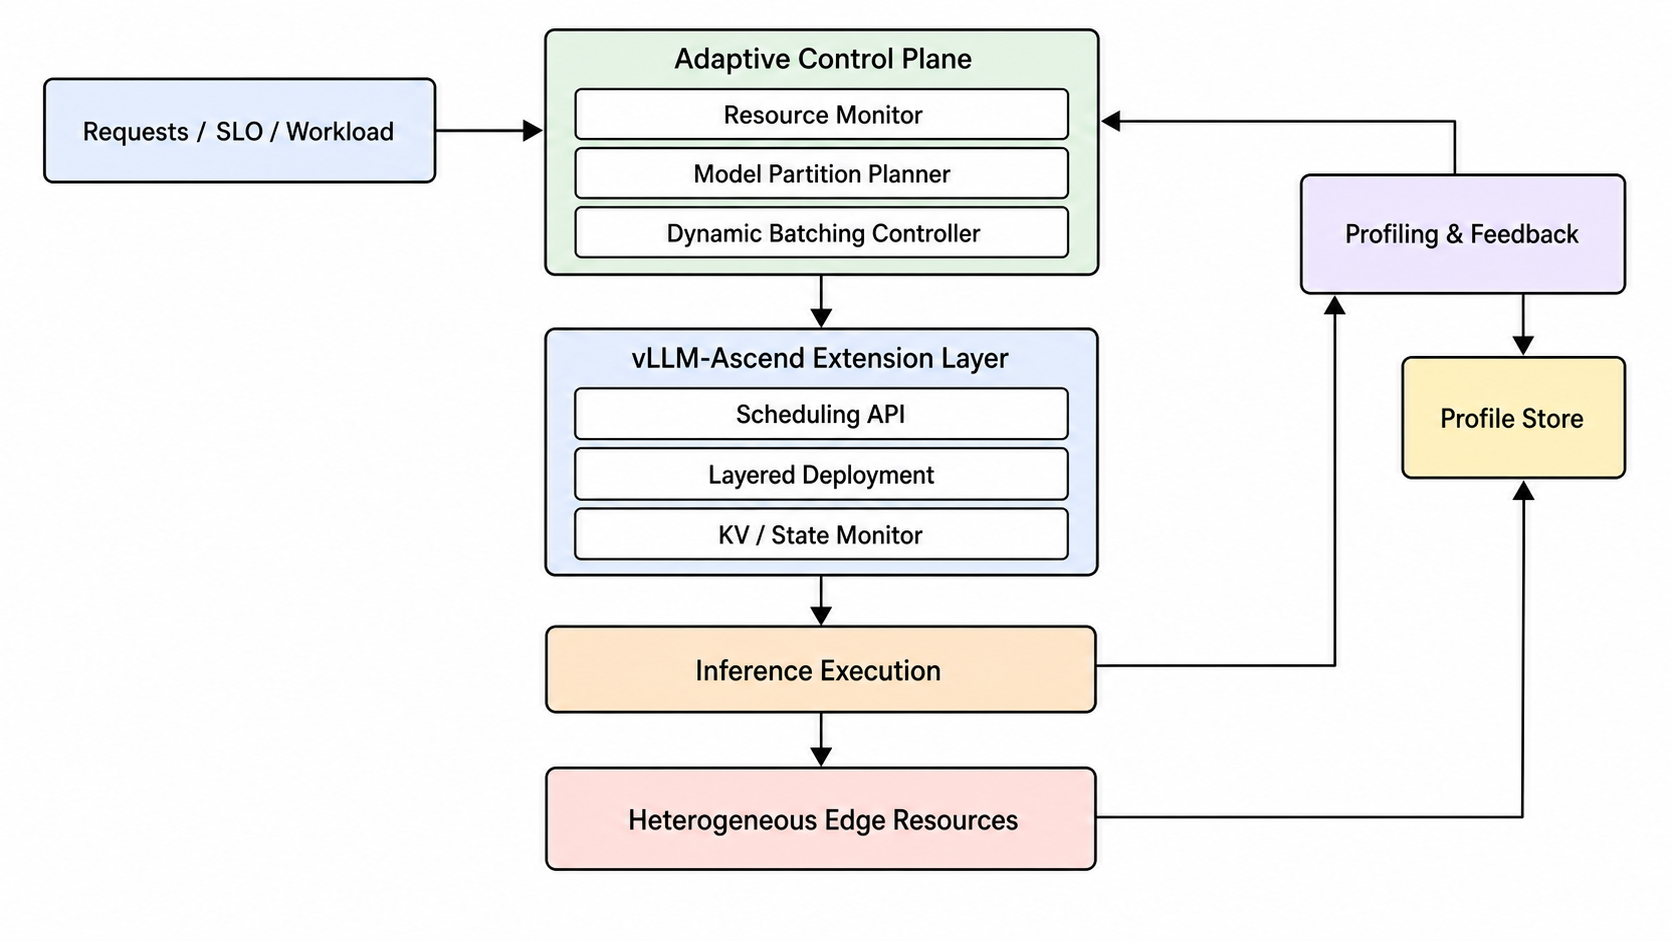
\includegraphics[width=\textwidth]{figures/ch8_engineering_architecture.png}
    \caption{面向 Ascend/CANN 验证环境的 CEC 推理工程框架}
    \label{fig:ch8-engineering-architecture}
\end{figure}

从请求路径看，业务请求从多个流量入口分别进入系统，携带 session ID、业务优先级、SLO、隐私标签、输入长度估计和上下文标识。入口层保持分布式接入方式，每个入口节点查询共享状态面并执行本地路由决策，同时接受控制面的全局约束和策略参数。入口层先判断已有 KV 或 prefix cache 位于哪个节点，再把节点显存、队列长度、链路状态和状态位置输入请求调度策略。若请求进入本地或近端实例，batching 策略决定其是否立即接纳、等待合批、进入长请求隔离队列或触发 chunked prefill；若请求需要跨节点执行，请求调度策略同时决定 KV 是本地读取、迁移、复制还是重算。

从反馈路径看，推理实例持续上报 TTFT、TPOT、ITL、E2E latency、active sequence 数、waiting queue 长度、KV block 占用、显存峰值、NPU 利用率、stage transfer time、链路 RTT/带宽和错误码。画像面将离线 profiling 与在线观测合并，形成 stage/link 代价、状态特征、动作效果、奖励和安全约束数据；状态面维护 KV owner、prefix block hash、session 入口变化和实例健康状态；控制面据此更新动态规划代价表、RL/bandit 策略、动作裁剪边界和请求路由代价。这个闭环需要为每次动作保留可追溯原因，例如选择某个切点和 placement、缩小 batch、迁移 KV 或重算 KV 时对应的状态、约束和收益估计。

\phantomsection
\subsection*{8.3 分阶段实现路线}
\addcontentsline{toc}{subsection}{8.3 分阶段实现路线}

第一阶段是 Ascend 层级切分执行能力。优先目标是让 CodeLlama34B、Qwen2-VL-7B-Instruct 等目标模型能够按连续 layer/block 切成多个 pipeline stage，并映射到 230T/64GB、70T/24GB、310P、910B4 或多机多卡 Ascend 节点上执行 \cite{huawei2026internal}。工程上需要解决四个接口：分段权重加载、stage 间 hidden state 传输、pipeline stage 启动参数和异常回退。接口稳定后，第四章的拓扑感知 layer-wise split 才能从规划结果转化为真实可部署方案，并进一步支撑 TP、EP、DP、PD 分离和 KV pool 等高阶动作。

第二阶段是 EdgeShard 风格的动态规划切分规划器。系统先对单实例、平均 layer split、固定 PP、固定 TP、PP+TP、layer sharding、context parallel、KV Cache Pool、PD 分离和 speculative decoding 等运行形态做离线 profiling，记录每层 latency、activation 大小、KV 增长、stage transfer cost、显存峰值和可支持并发，并用这些数据校准 stage 代价表、链路代价表和安全过滤器。切分规划的顺序应与第四章保持一致：先用动态规划搜索 layer-wise stage boundary、stage placement 和 pipeline balance；再判断单个 stage 是否需要叠加 TP，MoE 或组件化模型是否需要 EP，流量承载是否需要 DP；最后才把 PD 分离、KV Cache Pool 和 semantic/token-level collaboration 作为高阶候选。

第三阶段是分阶段增强的 RL/bandit 在线 batching 优化器。实现上先只训练参数自适应策略，保持框架默认请求顺序或 FIFO 不变，让策略根据并发、prompt 长度分布、KV 水位和 TTFT/TPOT/ITL 反馈调节 max running requests、max batched tokens、等待窗口、chunk size 和 prefill/decode quota。这样可以先确认收益是否来自 batching 参数本身。第二步再加入请求排序和准入控制，用 SLO slack、预测 prefill/decode 时间、KV 增长和对其他请求 ITL 的边际影响学习排序权重，使出队顺序同时反映业务紧迫度和系统边际成本。第三步再启用联合策略：短 prompt 和紧 SLO 时策略收紧 active set 与等待窗口，高并发且 slack 充足时扩大 token budget，长 prompt 或 VLM 比例升高时启用 chunked prefill 或长请求隔离，具备稳定 KV handoff 时才允许策略选择 PD 分离动作。

第四阶段是长期成本感知请求调度和 KV 管理。三个节点都应维护统一的节点负载、显存、网络和 KV 元数据；请求到达后，系统枚举目标计算节点以及 local、migrate、recompute 等状态处理动作，并先用 SLA 和 memory 约束过滤不可行动作。正常路由不只选择当前请求时延最低的节点，还要估计动作执行后 KV owner、节点负载、未来入口位置和后续 session 成本的变化。KV 管理应采用 block-level 索引和增量同步：迁移前先查询目标节点已有 prefix/KV blocks，只传输缺失部分；旧节点短期保留状态副本，以支持迁移失败、链路退化或负载突变时回退。

第五阶段是统一元数据驱动的协同控制。低频周期更新模型切分策略和服务能力布局，可按分钟级或配置变更事件触发；中频周期调节 batching 参数、admission threshold、prefill/decode quota 和实例分流，可按数秒到十秒级窗口触发；高频周期执行 request routing、workflow placement、KV migrate/recompute/local 动作和异常回退，可按单请求或 session 边界触发。三类决策必须共享同一状态视图：模型切分层输出 stage 容量和 KV handoff cost，batching 层输出队列等待和 KV 水位，请求调度层输出请求入口和状态位置。控制器重点处理三类冲突：切分带来的状态传输成本超过并行收益，batching 扩大等待窗口导致高优先级请求违约，路由因 KV 黏附远端节点造成长期跨节点通信。

\phantomsection
\subsection*{8.4 关键工程模块}
\addcontentsline{toc}{subsection}{8.4 关键工程模块}

第一个模块是 vLLM-Ascend / MindIE 接口适配层。它需要梳理模型加载、并行配置、scheduler、KV Cache 管理、metrics 暴露和错误码路径，并把底层能力转化为控制面可调用的动作接口。例如，模型切分策略输出的动作需要能够落到 stage 数、每个 stage 的 layer 范围、节点映射、tensor parallel degree、context parallel 开关、KV pool 策略和回退动作；batching 策略输出的动作需要能够落到 max running requests、max batched tokens、等待窗口、chunk size、prefill/decode quota 和 admission threshold；请求调度策略输出的动作需要能够落到目标实例、KV local/migrate/recompute、状态副本保留时间和失败回退路径。MindIE 可作为 Ascend 生态中生产化推理、调试、调优和迁移接口的参考底座 \cite{huawei2026mindie}；vLLM 的 OpenAI-compatible server 可作为服务入口和接口兼容性的参考 \cite{vllm2026openai}。

第二个模块是 Profile Store、Cost Table / Replay Buffer 与 Safety Guard。Profile Store 保存模型-硬件-拓扑的观测数据，包括 layer latency、activation、KV 增长、stage transfer cost、prefill/decode 吞吐、OOM 边界和链路状态；Cost Table 保存动态规划需要的 stage 代价、link 代价、显存约束和切换成本；Replay Buffer 保存 batching 与请求调度的状态、动作、奖励、违约和回退记录，用于离线训练、在线微调和策略回放评估；Safety Guard 保存显存上限、链路带宽下限、P99 TTFT 约束、动作冷却时间和回退条件。三者需要区分离线压测值和在线校正值：离线值用于生成初始代价表和安全边界，在线值用于修正当前窗口的动作裁剪、代价估计和奖励估计。这样可以避免系统在负载波动时盲目切换，也能避免长期使用过期画像。

第三个模块是在线策略决策器。模型切分策略只在低频周期或明显资源变化时输出动作，并设置冷却时间和最小收益阈值；batching 策略在中频周期更新参数、排序权重和准入阈值，但不直接替代 runtime 内部 token 调度；请求调度策略在高频周期处理每个 session/request 的目标节点和 KV 动作。三个决策器共享同一组约束：显存不溢出、SLA 不违约、链路带宽可承载、动作可启动、状态迁移成本可控。若安全过滤后可行动作为空，系统必须显式进入回退路径，例如降低并发、缩小 batch、回退固定 PP/TP、转发区域边缘或云端完整实例。

第四个模块是监控、审计和回退。验证环境中的算法收益必须能被复现，因此每次策略动作、batch 参数调整、请求迁移和 KV 重算都要记录触发状态、策略输出、安全过滤结果、奖励估计、最终动作和实际结果。监控指标至少包括 P90/P99 TTFT、TPOT、ITL、平均 E2E latency、SLA violation、满足 SLA 的 rps、最高并发用户数、显存峰值、OOM 次数、NPU 利用率、KV 命中率、状态迁移量和回退次数。对外报告时，应能区分收益来自层级切分策略、batching 参数自适应、请求排序策略、KV 迁移还是三者协同。

\phantomsection
\subsection*{8.5 验证路线}
\addcontentsline{toc}{subsection}{8.5 验证路线}

验证应按能力递进组织，先验证执行底座，再验证单类策略，最后验证协同闭环。第一组实验验证 Ascend 层级切分执行能力：比较单实例、平均 layer split、固定 PP/TP 和拓扑感知 layer-wise split，观察 OOM、P99 TTFT、TPOT、stage bubble、stage transfer time 和满足 SLA 的并发用户数。该组实验回答的是“Ascend 推理栈是否已经具备可执行的层级切分底座”。

第二组实验验证动态规划模型切分策略：在完成 profiling、stage/link 代价表和安全边界校准后，比较平均切分、固定 PP/TP、负载感知 placement、启发式拓扑感知 layer-wise split、EdgeShard 风格动态规划切分、动态规划加安全过滤和收益阈值。重点指标是满足 SLA 的请求处理数、最高并发用户数、显存峰值、通信开销、不可执行方案比例、pipeline bubble 和回退次数。这里的目标与第四章一致：相对于多节点平均切分基线，验证 goodput 和 SLA-constrained concurrency 是否有稳定提升 \cite{huawei2026internal}。

第三组实验验证 RL/bandit 在线 batching 优化器：先比较固定参数、离线调优参数、contextual bandit 和 actor-critic 参数自适应；再比较 FIFO、EDF/slack baseline、priority queue、边际代价排序和 RL 学习到的排序权重；最后在短 prompt、长 prompt、VLM 和多优先级混合 workload 上测试联合策略。指标应覆盖满足 SLA 的请求处理速度、平均 E2E latency、P99 TTFT、ITL 抖动、高优先级请求违约率、普通请求饥饿比例、策略切换次数和回退次数。

第四组实验验证长期成本感知请求调度和 KV 管理：比较就近执行、当前最小时延 Greedy、长期成本路由、长期成本路由加 block-level KV 管理。除 TTFT、E2E latency、吞吐和并发数外，还要统计用户移动后的累计通信时延、请求转发次数、KV 迁移/重算次数、状态传输量、prefix/KV 命中率和 session 节点切换次数。该组实验用于说明为什么 CEC 中的请求调度不能只看当前节点负载。

第五组实验验证协同控制：分别启用第四章切分策略、第五章 batching 策略和第六章请求调度但不共享状态，作为独立算法组合基线；再启用统一元数据但不做长期预测；最后启用完整的低频部署策略、中频 batching 策略、高频请求/状态路由闭环。扰动项包括链路带宽、RTT、可用显存、长 prompt 比例、移动用户比例和请求优先级分布。最终报告应同时给出性能收益和稳定性成本，尤其是策略切换频率、策略震荡、回退次数和状态传输开销。

\phantomsection
\subsection*{8.6 小结}
\addcontentsline{toc}{subsection}{8.6 小结}

工程结论是：面向 Ascend 验证环境的 CEC LLM 推理系统应先补齐层级切分执行底座，再把模型切分、batching 和请求调度分别实现为可观测、可回退、可解释的在线决策能力。第四章对应低频的动态规划混合切分部署；第五章对应中频的分阶段 RL/bandit batching 优化器；第六章对应高频的长期成本感知请求路由和 KV 管理；第七章则把三者收敛为统一元数据驱动的分层协同控制。

这样的工程路线与现有 vLLM-Ascend 能力并不冲突。vLLM-Ascend 继续负责模型加载、算子执行、KV 管理和实例内调度；外层系统负责画像、动态规划、策略学习、状态、路由、动作裁剪和回退。只有把“可执行动作接口”和“在线状态”放在同一个闭环中，前文提出的算法建议才会从综述中的方法对比，转化为验证环境中可以部署、压测和解释的工程方案。
